\documentclass{beamer}
\usepackage{pgfplots}   
\tikzset{%
	tdnn neuron/.style={
		rectangle,
		draw=black,
		fill=black!10,
		minimum height=0.5cm,
		minimum width=0.1cm 
	},
}
\begin{document}
	\begin{minipage}{\linewidth}
		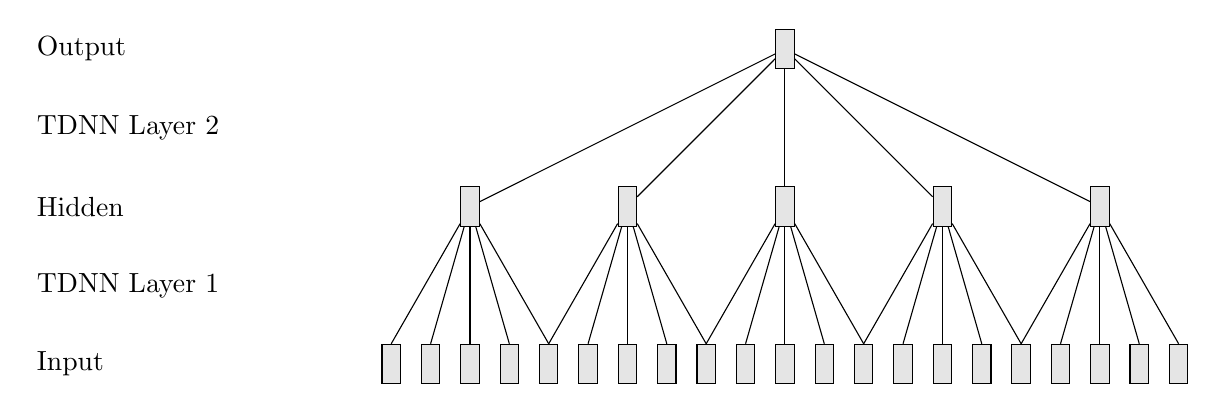
\begin{tikzpicture}
		% Layers
		\node[text width=4cm] at (-2,0) {Input};
		\foreach \m [count=\y] in {1,2,...,21}
		\node [tdnn neuron] (input-\m) at (\y*0.5,0) {};
		\node[text width=4cm] at (-2,1) {TDNN Layer 1};
		\node[text width=4cm] at (-2,2) {Hidden};
		\foreach \m [count=\y] in {1,2,...,5}
		\node [tdnn neuron] (hidden-1-\m) at (\y*2 - 0.5,2) {};
		
		\node[text width=4cm] at (-2,3) {TDNN Layer 2};
		\node[text width=4cm] at (-2,4) {Output};
		\foreach \m [count=\y] in {1}
		\node [tdnn neuron] (classify-\m) at (\y*0.5 + 5,4) {};
		
		%Edges
		\foreach \m [
		evaluate=\m as \nstart using int(((\m - 1) * 4) + 1),
		evaluate=\m as \nstep using int(((\m - 1) * 4) + 2),
		evaluate=\m as \nend using int(((\m - 1)* 4) + 5)] in {1,2,...,5}
		\foreach \i in {\nstart,\nstep,...,\nend}
		\draw (input-\i.north) -- (hidden-1-\m); % Error happens here. 
		
		\foreach \m in {1,2,...,5}
		\draw (hidden-1-\m) -- (classify-1);
		
		\end{tikzpicture}
	\end{minipage}
\end{document}